\section{Introduction}

\subsection{Contexte et motivation} %------------------------------------------------

\par Lotus est un logiciel d'analyse cinématique de la Liaison Au Sol (LAS) d'une voiture. Il permet notamment de définir les points caractéristiques des liaisons types d'une liaison au sol, de définir ces liaisons et d'étudier leur mouvement.

\par La démarche courante à l'EPSA combine une feuille de calcule Excel avec une génération des pièces par Catalogue CATIA:  cette méthode est très fonctionnelle mais également un peu lente. Une fois la configuration de points déterminée (sur Lotus), il est nécessaire d'ouvrir un tableau Lotus, de sélectionner manuellement les coordonnées des points, les copier-coller sur un fichier Excel dédié au paramétrage, enregistrer et fermer le fichier Excel, ouvrir le Catalog LASauto, ouvrir la fenêtre de mise à jour, sélectionner tous les composants dans l'arbre, lancer la mise à jour, attendre quelques minutes, fermer le Catalog, ouvrir l'assemblage de travail, faire une mise à jour et vérifier que tout s'est bien passé.

\par Ainsi, l'optimisation de la LAS d'un véhicule, typiquement pour un véhicule EPSA, nécessite de nombreuses itérations afin de tendre vers une géométrie et un confinement offrant une dynamique véhicule et un poids optimal. Il est donc primordial pour l'EPSA d'optimiser les mises à jour de LAS afin de gagner un temps considérable. Le but de ce projet est donc de permettre la mise à jour des composants à l'intérieur de l'Assemblage de Liaison au Sol du Véhicule dans Catia (Assemblage qui sera nommé plus tard simplement \texttt{Suspension}), mise à jour possible directement en lançant la Macro, par lecture du fichier Lotus, sans intervention manuelle sur l'Assemblage et sans utiliser la technologie de Catalog. Il est également souhaité de pouvoir définir de façon adaptée les pièces de l'assemblage de travail.

\par L'intérêt de ce rapport est donc de permettre la compréhension du code et de pouvoir utiliser la macro convenablement.


\subsection{Structure d'un fichier Lotus} %-------------------------------
\par Etant donné que ce projet est fondé sur l'étude d'un fichier Lotus au travers d'une macro Catia, la compréhension de la structure d'un tel fichier est importante.
Le fichier d'enregistrement de Lotus est de type \texttt{.dat}. Il s'agit d'un fichier Texte structuré afin de pouvoir enregistrer les différents paramètres d'un modèle Lotus. Le fichier est composé de différentes sections, ayant pour titre : \texttt{VERSION}, \texttt{PARAMETERS}, \texttt{TEMP\_GRAPHICS}, \texttt{TEMP\_SETTINGS}, \texttt{FRONT SUSPENSION}, \texttt{REAR SUSPENSION},
\texttt{COMPLIANCE} et
\texttt{MODAL}. Tout ceci est résumé dans la Fig.\ref{fig:structure_lotus}

\begin{figure}
    \centering
    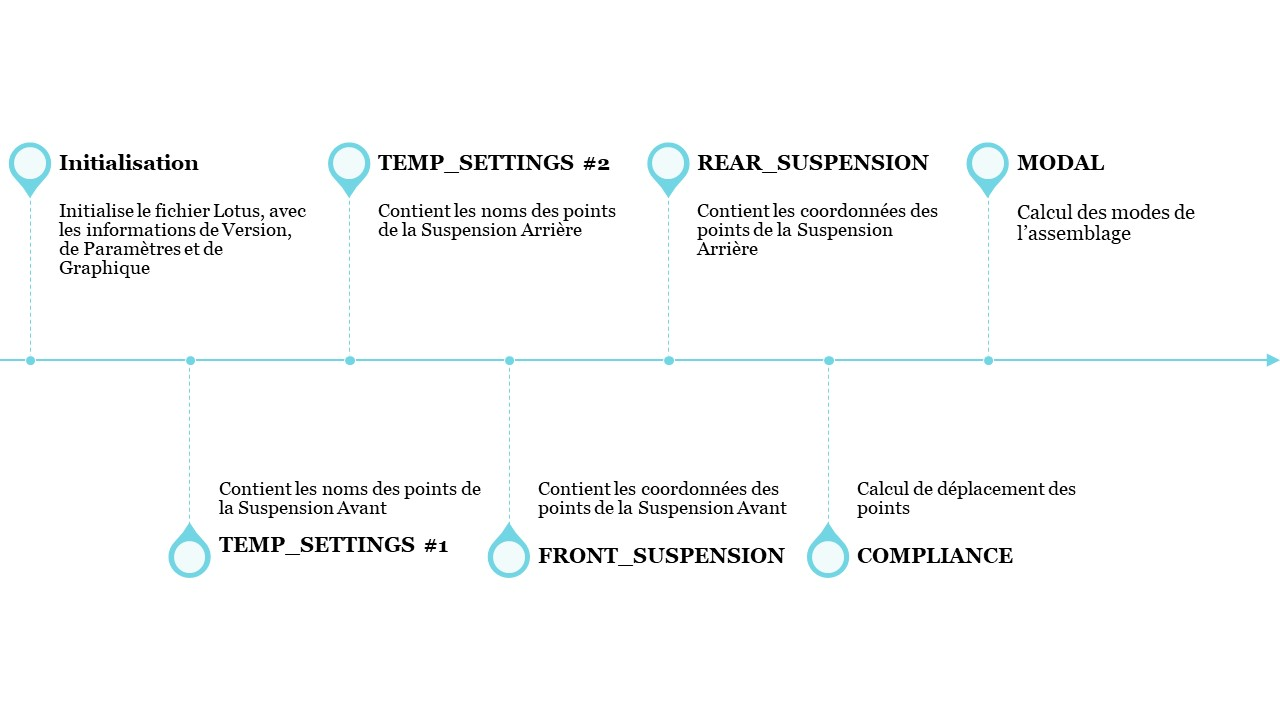
\includegraphics[width=\linewidth]{img/Structure_Fichier_Lotus.jpg}
    \caption{Structure d'un Fichier Lotus}
    \label{fig:structure_lotus}
\end{figure}

\newpage
\par Ainsi, Lotus définit des modèles d'architecture pour différentes géométries de Suspension. Une géométrie de Suspension modifie tout simplement ce modèle et enregistre les nouvelles coordonnées des points dans un fichier \texttt{.dat}. \par Dans la section \texttt{TEMP\_SETTINGS} de ce fichier, on retrouve la définition des pièces de la suspension ainsi qu'une liste des points du modèle de suspension choisi.
\par Dans la section \texttt{FRONT SUSPENSION} et \texttt{REAR SUSPENSION}, on retrouve les coordonnées des points du modèle de suspension (respectivement pour le train avant et arrière).
\par Ce sont ces deux types de sections qui vont nous intéresser.


\paragraph{Structure de la section \texttt{TEMP\_SETTINGS}} %----------------

\par Un exemple de section \texttt{TEMP\_SETTINGS} d'un fichier Lotus est présenté en Fig. \ref{fig:temp_settings}. Après l'entête (ligne 1) et la description du template utilisé pour la création du modèle Lotus (lignes 2 et 3), on retrouve une série de nombres. Le premier indique le nombre de pièces dans le modèle et le deuxième le nombre de points dans le fichier. Dans l'exemple de la Fig. \ref{fig:temp_settings}, le nombre de pièces est 6 et le nombre de points est 2. Le nom de chaque pièce est listé de la ligne 5 à la ligne 10, suivi de la définition de chaque point dans le modèle. On s'intéresse ici seulement à la lecture du nom du point : on lit donc la ligne 11 ( pour le point numéro 1) et on saute 8 lignes pour arriver à la définition du point numéro 2 (ligne 20).

\begin{figure}
    \centering
    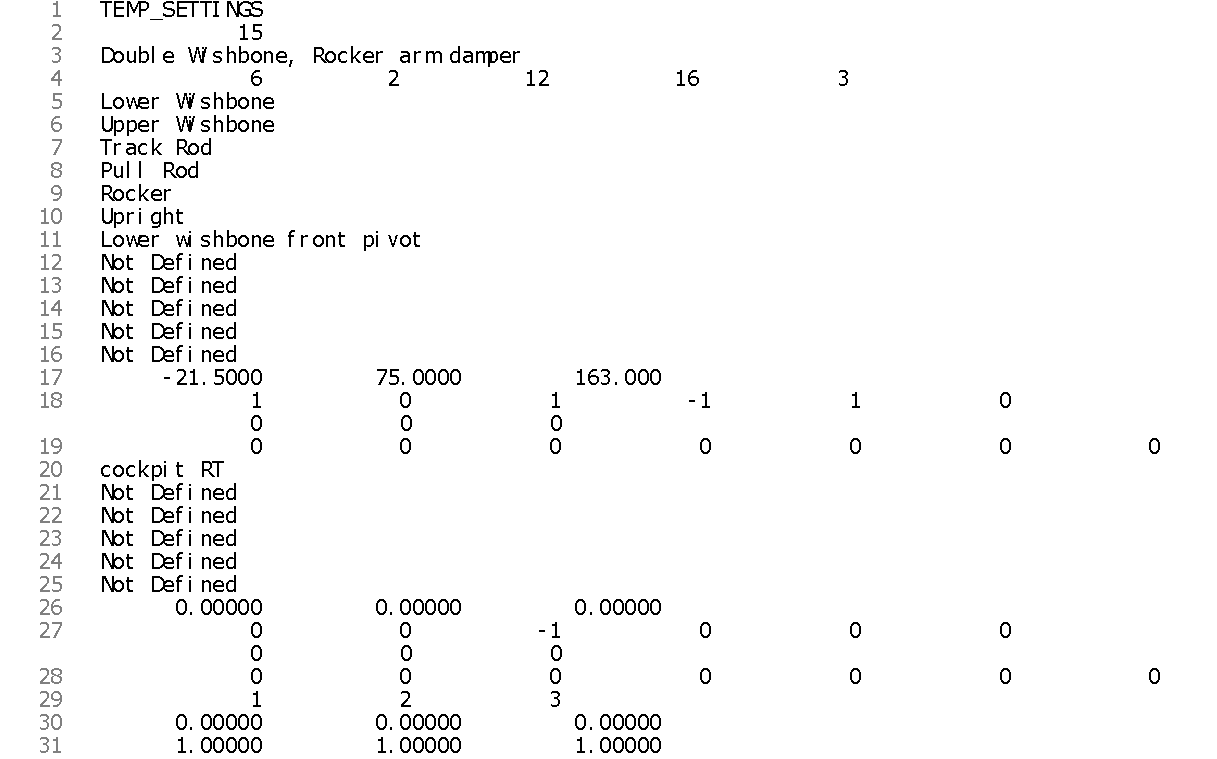
\includegraphics[width=\linewidth]{fichiers/temp_settings.pdf}
    \caption{Structure de la section \texttt{TEMP\_SETTINGS} avec 2 points}
    \label{fig:temp_settings}
\end{figure}


\paragraph{Structure de la section \texttt{FRONT (REAR) SUSPENSION}} %---------------------

\par Un exemple de section \texttt{FRONT SUSPENSION} est présenté en Fig. \ref{fig:frontSuspension}. Après l'entête (ligne 3), on retrouve le code du template utilisé (ligne 2 Fig. \ref{fig:temp_settings}) et ensuite un tableau de coordonnées des points du Template. Cet exemple utilise un Template avec 27 points, les coordonnées sont donc listées dans les lignes 5 - 31

\begin{figure}
    \centering
    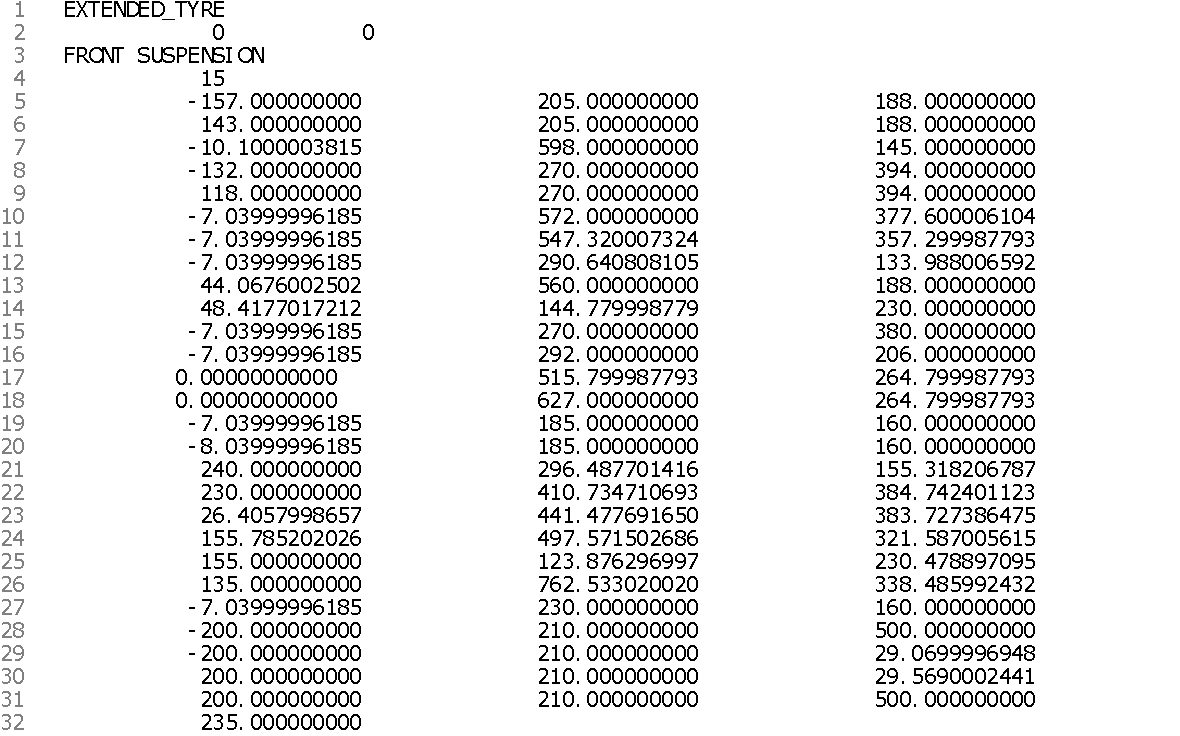
\includegraphics[width=\linewidth]{fichiers/front suspension.pdf}
    \caption{structure de la section \texttt{FRONT SUSPENSION}}
    \label{fig:frontSuspension}
\end{figure}

\newpage
\subsection{Besoins du système LAS vis à vis de la maquette} % ----------------------

\par Les besoins du système liaison au sol sont résumés ci-dessous, représenté par d'abord le pseudo-code de l'application puis le cahier des charges qu'a dû respecter notre application.\\

\paragraph{Pseudo-code}
\noindent\textit{Inputs, obtenu grâce à l'utilisateur, après lancement de l'Userform} (cf Section \ref{interf_graph})
\begin{itemize}
    \item Path du fichier Lotus .dat
    \item Path du Wireframe.CATProduct contenant LotusPoint.CATPart
    \item Paths d'autres Products à mettre à jour
\end{itemize}
\textit{Running}
\begin{itemize}
    \item \textbf{Appel du module LectLotus} (cf Section \ref{lect_lotus}),
        \subitem{- Lecture du fichier .dat}
        \subitem{- Récupération, dans des listes, des noms et des coordonnées des points du train avant et arrière}
    \item \textbf{Appel du module MajCatia} (cf Section \ref{majcatia}),
        \subitem{- Ouverture de fichier LotusPoint.CATPart}
        \subitem{- \textbf{Pour} i=1 à len (nom\_points train avant)}
            \subsubitem{- Si le point existe déjà :}
                \subsubsubitem{Mise à jour de ses coordonnées}
            \subsubitem{- Sinon :}
                    \subsubsubitem{Création du point}
        \subitem{- \textbf{Pour} i=1 à len (nom\_points train arrière)}
            \subsubitem{- Si le point existe déjà :}
                \subsubsubitem{Mise à jour de ses coordonnées}
            \subsubitem{- Sinon :}
                    \subsubsubitem{Création du point}
        \subitem{- Mise à jour de LotusPoints.CATPart}
        \subitem{- Mise à jour de Wireframe\_Definition.CATProduct}
        \subitem{- Mise à jour des autres Products sélectionnées par l'utilisateur}
        \subitem{- Fermeture de tous les fichiers Catia}
\end{itemize}
\textit{Outputs}
\begin{itemize}
    \item Nombre de points créés et mis à jour pour le train avant
    \item Nombre de points créés et mis à jour pour le train arrière
\end{itemize}

\paragraph{Cahier des charges de l'application VBA} %----------------------------

\begin{itemize}
    \item Offrir une interface graphique à l'utilisateur
    \item Permettre à l'utlisateur la sélection, par explorateur de fichiers, des documents qu'ils souhaitent utilisés, mettre à jour, etc
    \item Permettre la lecture des points et leurs coordonnées depuis un fichier Lotus \texttt{.dat} sélectionné à partir de l'explorateur de fichiers
    \item Mettre à jour le fichier Catia automatiquement et d'autres fichiers Catia souhaités par l'utilisateur
    \item Indiquer le nombre d'opérations sur les coordonnées effectuées à l'utilisateur afin qu'il puisse vérifier la bonne exécution du programme
    \item Anticiper quelques erreurs classiques et les indiquer à l'utilisateur quand il les exécute
    \item Pouvoir réutiliser les fichiers de conception détaillée de la saison 2020
\end{itemize}{}